\documentclass[sigconf]{acmart}
\settopmatter{printacmref=false}

\usepackage{amsmath}
\usepackage{graphicx}
\usepackage{threeparttable}
\usepackage{booktabs}
\usepackage{pifont}

\usepackage{xeCJK}
\setCJKmainfont{SimSun}

\title{Ordovician: Mixed-Precision Quantized Inference Accelerator for Sparse Transformers on CPU/FPGA Co-Porcessing System}

\author{Lei Gong}
\affiliation{
	\institution{University of Science and Technology of China}
	\city{Hefei}
	\country{China}
}

\acmConference[ShortName]{FullName}{Date}{Location}
\acmDOI{DOI}

\begin{document}
	
	\begin{abstract}
	\end{abstract}
	
	\keywords{Vision-Language Model, Mixed-Precision Quantization, Contextual Sparsity, Embedded Platform, CPU/FPGA Co-Processing}
	
	\maketitle
	
	\section{Introduction}
	随着多模态人工智能的发展，视觉语言模型（Vision-Language Models, VLM）在视觉理解、视觉问答、多模态推理以及人机交互等任务中展现出强大的能力。相比仅处理文本的模型，VLM 能够综合处理视觉与文本信息，从而更好地理解复杂的真实世界环境。因此，VLM 在边缘端平台上部署的需求日益增长，尤其是在自动驾驶等资源受限的嵌入式场景中。

	目前，边缘侧推理计算通常采用以下几种部署方式：一是基于云端 GPU 的集中式推理服务，通过远程调用完成推理计算；二是基于高性能 GPU 的桌面端部署，用于满足较低延时需求；三是在嵌入式设备上进行本地推理。相较于前两中部署方式，在资源受限的嵌入式环境中，特别是在存储容量和访存带宽方面的严格限制下，实现性能、功耗满足要求的 VLM 部署仍然面临重大挑战，这在很大程度上限制了 VLM 的实际落地。

	桌面端和云端借助模型量化和神经元动态稀疏化提升 LLM 部署效能的方法提供了优化思路，但直接引入嵌入式端的 VLM 部署仍存在难点。模型量化通过将模型参数和激活值从浮点精度压缩为低比特表示，例如 INT8、INT4 等，可以显著减少模型存储容量并提升推理计算效率。然而，现有硬件平台通常仅支持固定精度计算，对模型的统一精度量化使得低比特量化对模型精度影响较大，无法充分利用不同层或不同模块的精度特性充分压缩数据大小。除了量化技术之外，神经元动态稀疏化通过剪枝或结构化稀疏化技术，可以减少模型中不重要的权重参数，从而降低矩阵乘法计算量并提高推理效率。然而，当前大多数通用计算平台在执行稀疏矩阵计算时难以充分利用稀疏结构，往往仍然按照密集矩阵进行计算，从而无法获得理想的性能提升。综上所述，现有嵌入式平台在执行大模型推理时，往往受到通用硬件架构限制而无法充分利用量化和稀疏性优化带来的计算量与实时性地提升。
	
	为了解决上述问题，本文提出了嵌入式端的 CPU/FPGA 耦合的 VLM 推理计算架构，并将其应用于 LLaVA-7B 视觉语言模型的推理部署。系统在算法层面，将混合精度量化与动态神经元稀疏进行结合，改进了传统稀疏性预测方法，提出了新的推理范式；在硬件层面，为混合精度矩阵乘法和稀疏矩阵乘法计算提出了适配算法优化的专用 FPGA 硬件架构。
	
	\section{Background and Motivation}

	\subsection{FPGA-Based VLMs}
	
	VLM 在多模态任务中展现出了卓越的性能，但将其部署于资源受限的嵌入式环境中仍面临巨大挑战。这种困难主要源于 VLM 庞大的参数规模和密集的计算需求，导致在低存储容量和低内存带宽的边缘设备上，难以实现低延迟与低能耗的推理。
	
	在 FPGA（Field-Programmable Gate Array）上部署 VLM 为解决这一部署瓶颈提供了极具潜力的途径。首先，在实现低延迟方面，FPGA 允许研究人员打破传统冯·诺依曼架构的限制，人为设计高度定制化、深层流水线化的推理计算通路。通过将连续的计算层映射到空间架构上，并精确控制片上 SRAM 的数据流转与访存调度，FPGA 可以显著减少对片外 DRAM 的依赖，从而消除通用处理器在密集 I/O 时的访存延迟瓶颈。
	
	其次，在实现低能耗方面，FPGA 具有天然的细粒度硬件可编程性。与通用 CPU 或 GPU 相比，FPGA 剔除了复杂的指令获取、译码以及动态分支预测等额外开销。它的纯数据驱动计算模式使得逻辑门电路仅在数据到达时发生翻转，配合定制化的低比特数据路径，极大地降低了单位算力的动态功耗。
	
	因此，基于 FPGA 的 VLM 部署方案能够有效应对边缘计算的严苛约束。近年来，学界与业界已有大量成功案例证实了该路径的可行性，例如基于 FPGA 的高效 Transformer 加速架构通过软硬件协同设计，在保持模型精度的同时，实现了数量级上的能效比提升（例如 FlightLLM [1] 等针对大模型底层硬件行为优化的定制框架）。

	\begin{figure}[htbp]
		\centering
		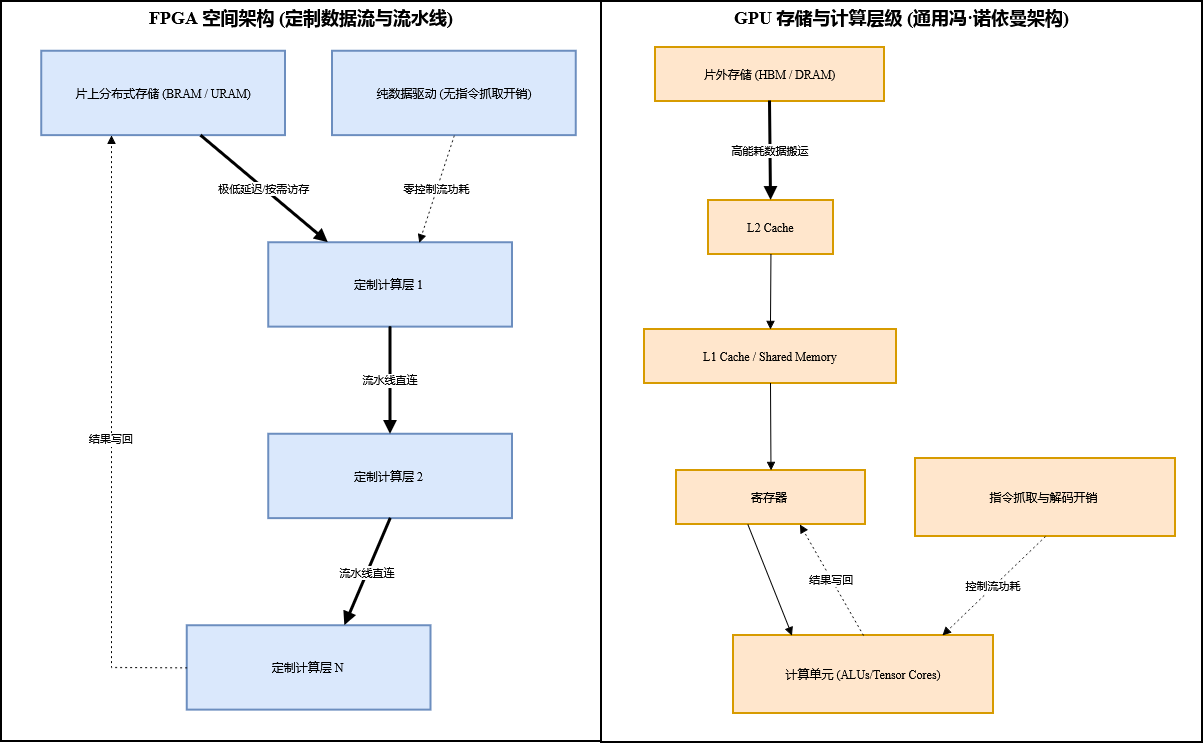
\includegraphics[width=0.95\linewidth]{fig/picture1.png} 
		\caption{通用 GPU 与定制 FPGA 加速器在存储层级与执行范式上的对比。GPU 架构（右）依赖复杂的存储层级，导致较高的数据搬运和指令开销。相反，基于 FPGA 的数据流架构（左）利用分布式片上 SRAM 和定制流水线，实现了低延迟、高能效的 VLM 推理。}
		\label{fig:fpga_gpu}
	\end{figure}

	\subsection{Mixed-Precision Quantization}

	为了进一步缓解 VLM 推理过程中的“内存墙”与计算瓶颈，量化技术，特别是混合精度量化成为了不可或缺的手段，它在提升大模型推理速度与降低能耗方面发挥了决定性作用。

	传统的统一低比特量化（如全局 INT4 或 INT8）虽然能大幅压缩模型体积，但往往会造成不可接受的精度损失，尤其是在大语言模型中普遍存在的激活值异常点难以被有效处理。混合精度量化通过对模型不同层次、不同模块（如权重、激活值、KV Cache）的敏感度进行细粒度分析，为不同部分分配最合适的位宽。例如，对绝大部分数值分布平缓的权重采用极低比特（如 4-bit 甚至更低）进行存储以加速内存读取，而对包含关键上下文信息的激活值或异常通道保留较高的精度（如 8-bit 或 16-bit 浮点），从而在不损失生成质量的前提下最大化硬件执行效率。
	
	在近三年的研究中，混合精度与高效量化技术取得了突破性进展。业界广泛采用的 AWQ (Activation-aware Weight Quantization) [2] 通过保留极少量（约 1\%）显著权重的精度，实现了高效的 4-bit 权重推理。SmoothQuant [3] 则通过数学等价变换将激活值的量化难度转移到权重上，成功实现了无损的 W8A8（权重 8-bit，激活 8-bit）量化，极大降低了推理能耗并提升了吞吐量。此外，最新的 BitNet b1.58 [4] 探索了 1-bit（三元参数）架构，彻底去除了浮点乘法运算，这与 FPGA 极度契合，为未来极低功耗的硬件原生部署指明了方向。

	\begin{figure}[htbp]
		\centering
		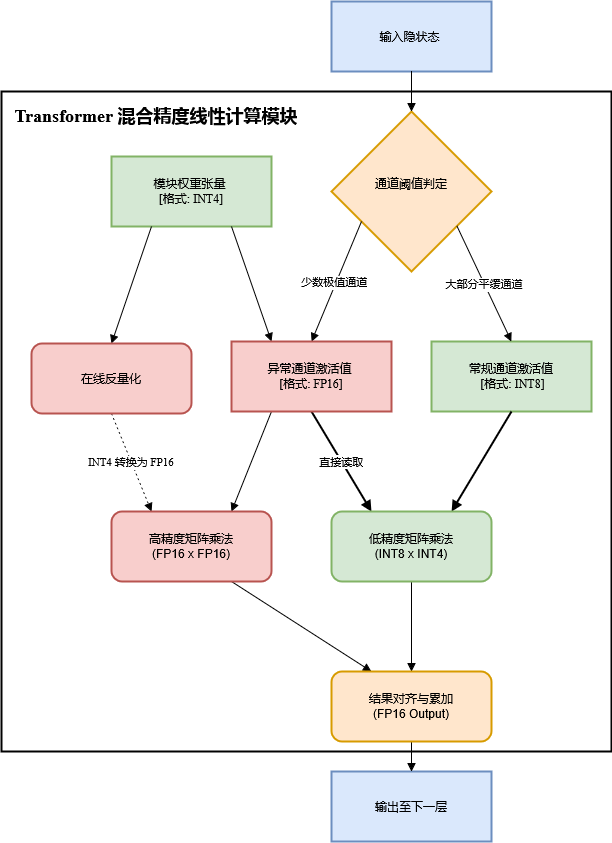
\includegraphics[width=0.95\linewidth]{fig/picture2.png} 
		\caption{Transformer 块中的混合精度量化策略示意图。线性层权重以 INT4 格式存储。激活值根据异常点检测进行动态分离：少数极值通道在 FP16 下计算以保持模型精度，而大部分常规通道则在 INT8 下处理，以最大化硬件执行效率。}
		\label{fig:mixed_precision}
	\end{figure}
	
	\subsection{Contextual Sparsity}
	
	在大规模模型的推理计算中，针对特定输入，模型通常表现出高度的上下文稀疏性。这意味着模型只需动态激活少量的多头注意力（MHA）和多层感知机（MLP）参数，便可近似甚至完全复现稠密模型的输出结果。具体而言，MHA 的稀疏性主要源自 Token 嵌入空间的相似性与注意力矩阵的聚类行为（如 Attention Sinks 现象）；而 MLP 层的稀疏性则来自激活函数（如 ReLU 或 SwiGLU）引入的输入依赖性，大量神经元在特定输入下输出趋近于零。
	
	基于这一观察，我们可以通过采集模型推理过程中的激活值数据，构建表征稀疏性模式的参数样本。利用这些样本，可以训练简单的全连接神经网络分类器，并使用交叉熵损失函数优化，从而构建出前瞻预测器 [5]。在实际推理过程中，该预测器能够根据当前层的中间数据，轻量且提前地预测出后续计算层的稀疏激活模式。
	
	这种动态路由机制使得底层硬件能够在不损失模型泛化性能与上下文学习能力的前提下，直接跳过大量冗余参数的加载与计算。近期如 PowerInfer [6] 等研究进一步利用了这种神经元激活的局部性，结合硬件访存特性，实现了计算资源的精准按需分配，从而极大地提升了模型在边缘设备上的推理效率。
	
	\section{Ordovician Overview}
	
	Ordovician 是一种面向资源受限环境的 CPU/FPGA 耦合 VLM 推理加速系统。系统充分利用 FPGA 在低功耗计算和定制化计算通路方面的优势，同时结合 CPU 在任务控制调度、动态内存管理以及输入输出处理上的灵活性，在有限硬件资源条件下实现低延迟、低功耗的 VLM 推理部署。与传统端到端的大模型推理框架不同，Ordovician 并不负责完整的模型执行流程，而是专注于模型中计算开销最高、资源消耗最大的 Transformer 核心计算部分；对于 tokenizer 编码、token 构建、logits 向量计算以及最终输出 token 解码等辅助任务，则交由其他计算部件完成。从系统接口层面来看，Ordovician 表现为一个“读取输入 token、返回输出 token”的 CPU 程序接口，而其内部则通过 CPU/FPGA 协同执行机制完成 Transformer Block 的高效推理计算。图~\ref{fig:overview}展示了 Ordovcian 在 LLaVA Vison Tower 推理计算中发挥的作用。
	
	\begin{figure}[htbp]
		\centering
		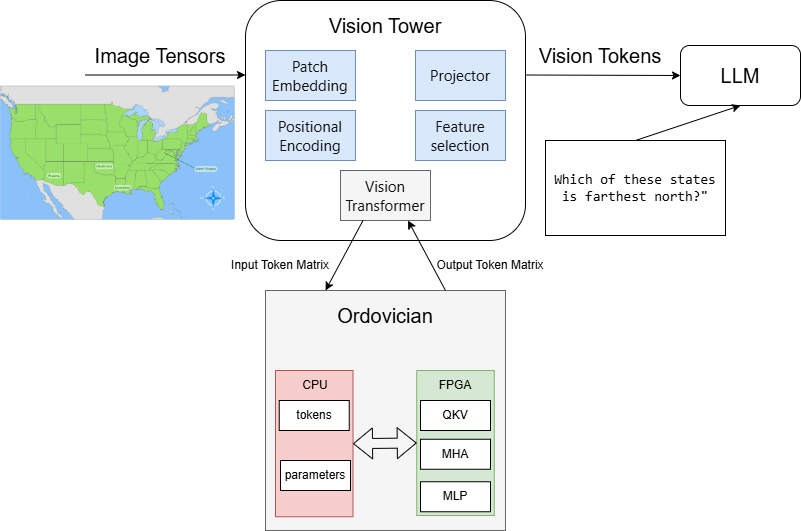
\includegraphics[width=\linewidth]{fig/overview.png}
		\caption{Ordovcian 在 LLaVA Vison Tower 推理计算中发挥的作用。在 LLaVA 的 Vision Tower 推理过程中，输入图像首先被转换为 Image Tensors，并依次经过 Patch Embedding、Positional Encoding、Vision Transformer、Feature Selection 与 Projector 等计算阶段生成输出张量 Vision Tokens，其中 Ordovician 以“读取输入 token、返回输出 token”的 CPU 程序接口形式嵌入至整个推理流程中，专门负责 Vision Transformer 部分多个 Transformer Block 的高效推理计算，从而利用 CPU/FPGA 协同执行架构实现 Vision Transformer 模块的低延迟、低功耗推理计算。}
		\label{fig:overview}
	\end{figure}
	
	在 Ordovician 中，CPU 主要负责输入输出 token 及模型参数的内存管理、数据调度与推理流程控制，而 FPGA 则作为 Transformer 算子的专用加速引擎，负责 MHA、MLP 等 Transformer 核心计算任务。
	
	由于 FPGA 片上 BRAM/URAM 存储资源有限，Ordovician 无法在片内完整缓存所有 Transformer 参数，由 CPU 承担参数服务器的角色，在 FPGA 推理过程中按需向提供当前 Transformer Block 所需的模型数据，能够在资源受限环境下实现大规模模型参数的动态加载与高效管理，并有效降低片上存储压力。
	
	此外，将 FPGA 作为 CPU 的专用协处理器执行 Transformer 核心推理计算，能够充分发挥 FPGA 在定制化数据流架构、低功耗并行计算以及细粒度硬件控制方面的优势；Ordovician 在 FPGA 上设计的混合精度矩阵乘法模块与稀疏矩阵乘法模块，便能有效缓解传统通用处理器在量化与稀疏化模型推理过程中存在的资源利用率不足与无效计算开销问题，使模型量化与神经元稀疏化带来的理论优化收益能够更充分地转化为实际推理性能提升。

	\subsection{Architecture and Workflow}
	
	图 X 展示了本文提出的 CPU–FPGA 耦合 VLM 推理系统整体架构，其由 CPU 侧控制模块、FPGA 推理加速器以及 CPU/FPGA 协同通信机制三部分组成。整个推理流程采用 token 迭代执行方式，逐层完成 Transformer Block 的推理计算。

	\textbf{CPU-side Runtime Manager}：
	在推理开始前，CPU 首先为输入 token、输出 token 、缓存 token 以及 KV Cache 申请对应内存空间，随后加载当前 Transformer Block 所需的模型参数、预训练的稀疏性预测器参数（Step \ding{172}）；完成数据准备后，CPU 启动 FPGA 加速算子，并正式开始该 Transformer Block 的推理计算流程（Step \ding{172}）。

	\textbf{FPGA-based Transformer Accelerator}：
	FPGA 侧实现了面向 Transformer 的专用推理流水线，负责执行多个 Transformer Block 的核心计算任务。每个 Block 包括 Attention 模块与 MLP 模块两部分。
	
	在 Attention 阶段，加速器首先完成输入 token 的 QKV 矩阵投影，并进一步执行 Attention Score 计算与 Value 聚合操作（Step ③）。针对矩阵运算特征，系统采用向量化 PE（Processing Element）阵列实现高并行度 MAC 运算，并通过片上流水线降低中间数据访存开销。
	
	与此同时，系统并行启动 MLP 激活预测模块，对下一阶段 FFN 中可能被激活的神经元进行预测（Step ④）。该预测模块基于当前 token 的中间特征生成稀疏激活掩码，仅保留高概率活跃神经元。
	
	进入 MLP 阶段后，FPGA 根据预测结果有选择地请求 CPU 中对应的权重参数，并执行稀疏矩阵乘法运算（Step ⑤）。由于大量非激活神经元被提前跳过，加速器能够显著减少计算量与 DDR 访存压力。MLP 输出结果随后与残差连接融合，并作为下一 Transformer Block 的输入继续迭代执行。
	
	在完成全部 Transformer Block 后，FPGA 对最终 token 执行归一化与 logits 计算，并将结果返回至 CPU（Step ⑥）。CPU 根据 logits 结果选择输出 token，并继续后续自回归生成过程，直至推理结束。
	
	\textbf{CPU/FPGA communication}：
	CPU 在调用 FPGA 算子时，除向 FPGA 传输输入输出 token、KV Cache 以及模型参数等相关数据地址外，还会附加当前正在执行的 Transformer Block 编号；每当 CPU 接收到 FPGA 算子执行完成信号后，便更新当前 Transformer Block 所需的模型参数，并再次启动 FPGA 算子以继续执行下一 Transformer Block 的推理计算，直至所有 Transformer Block 推理完成后返回最终输出 token 数据。
	
	对于 FPGA 算子而言，其在获取 CPU 侧提供的数据地址的同时，也会接收当前 Transformer Block 编号：若当前处理的是首个 Transformer Block，则首先将 CPU 输入 token 加载至 FPGA 片上 token 缓存；若当前已完成全部 Transformer Block 的推理计算，则将片上 token 缓存中的最终结果写回 CPU 输出 token；而在其余情况下，则从 CPU 侧 缓存 token 中读取中间 token 数据，并在完成当前 Block 推理后重新写回对应缓存区域，以供后续 Transformer Block 继续使用。
	
	\subsection{Single Transformer Block Example}
	
	图 X 展示了 LLaVA-7B Vision Tower 中 Full-Attention 单个 Transformer Block 在 Ordovician 中的推理执行流程。
	
	FPGA 侧加速算子主要由 QKV、MHA 以及 MLP 三个核心计算模块组成。其中，QKV 模块负责完成输入 token 矩阵向 Query（Q）、Key（K）与 Value（V）矩阵的线性投影计算。考虑到 FPGA 片上 BRAM/URAM 存储资源有限，Ordovician 仅在 FPGA 侧保留 Q 矩阵相关数据，而将生成的 KV 矩阵写回 CPU 侧的 KV Cache 中进行存储与管理。尽管在 Vision Tower 的 Full-Attention 推理场景下，QKV 矩阵通常可以在单次推理过程中同步完成计算，因此严格意义上并不存在 KV Cache 的长期复用需求，但 Ordovician 仍保留了 KV Cache 的整体架构设计：一方面，这是针对 FPGA 极其有限片上存储资源所做出的工程性权衡，以减少 KV 数据对片内缓存空间的占用；另一方面，该设计也能够更好兼容常见 Transformer Decoder 的自回归推理流程，从而为 Ordovician 在后续开发中支持不同类型的 Transformer 推理任务预留统一的数据通路与缓存管理机制。
	
	在 MHA 模块中，Ordovician 负责完成 Attention Score 的生成、归一化以及最终 Attention 输出的计算；在 MLP 模块中，则进一步完成双层线性投影运算，并生成最终输出 token。QKV、MHA 与 MLP 三个核心模块在执行矩阵乘法运算时，均会调用混合精度矩阵乘法模块，以实现对 INT4、INT8 与 FP16 等不同精度数据的统一计算支持；此外，MLP 模块还会进一步调用稀疏矩阵乘法模块，结合神经元稀疏性预测结果，仅对激活神经元执行稀疏矩阵计算，从而实现对 MLP 层的稀疏化推理优化，并有效降低整体计算量与外部访存开销。
	
	随后，MLP 稀疏预测模块根据当前特征预测下一层神经元的激活状态。假设某一层共有 8 个神经元，其中仅预测神经元 2、5 与 7 会被激活，则 FPGA 仅请求这部分神经元对应的权重参数，而跳过其他非活跃神经元。
	
	在执行阶段，FPGA 稀疏矩阵计算单元仅对神经元 2、5 与 7 执行乘加运算，并通过向量化流水线完成部分和累积。与此同时，CPU 通过 DMA 按需传输相关参数数据，实现计算与数据传输重叠。最终，加速器对所有激活神经元输出进行融合，生成该 MLP 层的最终输出结果。
	
	与传统稠密 Transformer 推理相比，该方法避免了大量无效神经元计算与参数访存。在大规模 VLM 中，由于 FFN 层参数通常占据模型总参数的大部分，本工作提出的稀疏感知 CPU–FPGA 协同机制能够有效降低 FPGA 存储压力与系统功耗，同时提升整体推理吞吐率。
	
	\section{混合精度乘加树计算阵列}
	
	在实现上述推理架构的过程中，首先需要解决混合精度计算的支持问题。由于量化模型通常采用多种不同精度表示，因此需要设计能够支持多种精度的乘加计算逻辑。针对这一挑战，项目在 FPGA 上构建了统一的整型与浮点计算通路，设计实现了可支持 INT4、INT8 和 FP16 三种精度的乘加树计算单元。在此基础上，进一步实例化了 4 个乘加树阵列，每个阵列内部集成 64 组可流水线化、并行运行的乘加树单元，共同构成 16×16 的矩阵乘法计算阵列。这一设计使得计算模块能够在不同精度模式之间灵活切换，从而高效支持混合精度量化模型的推理计算。
	
	\begin{figure}[htbp]
		\centering
		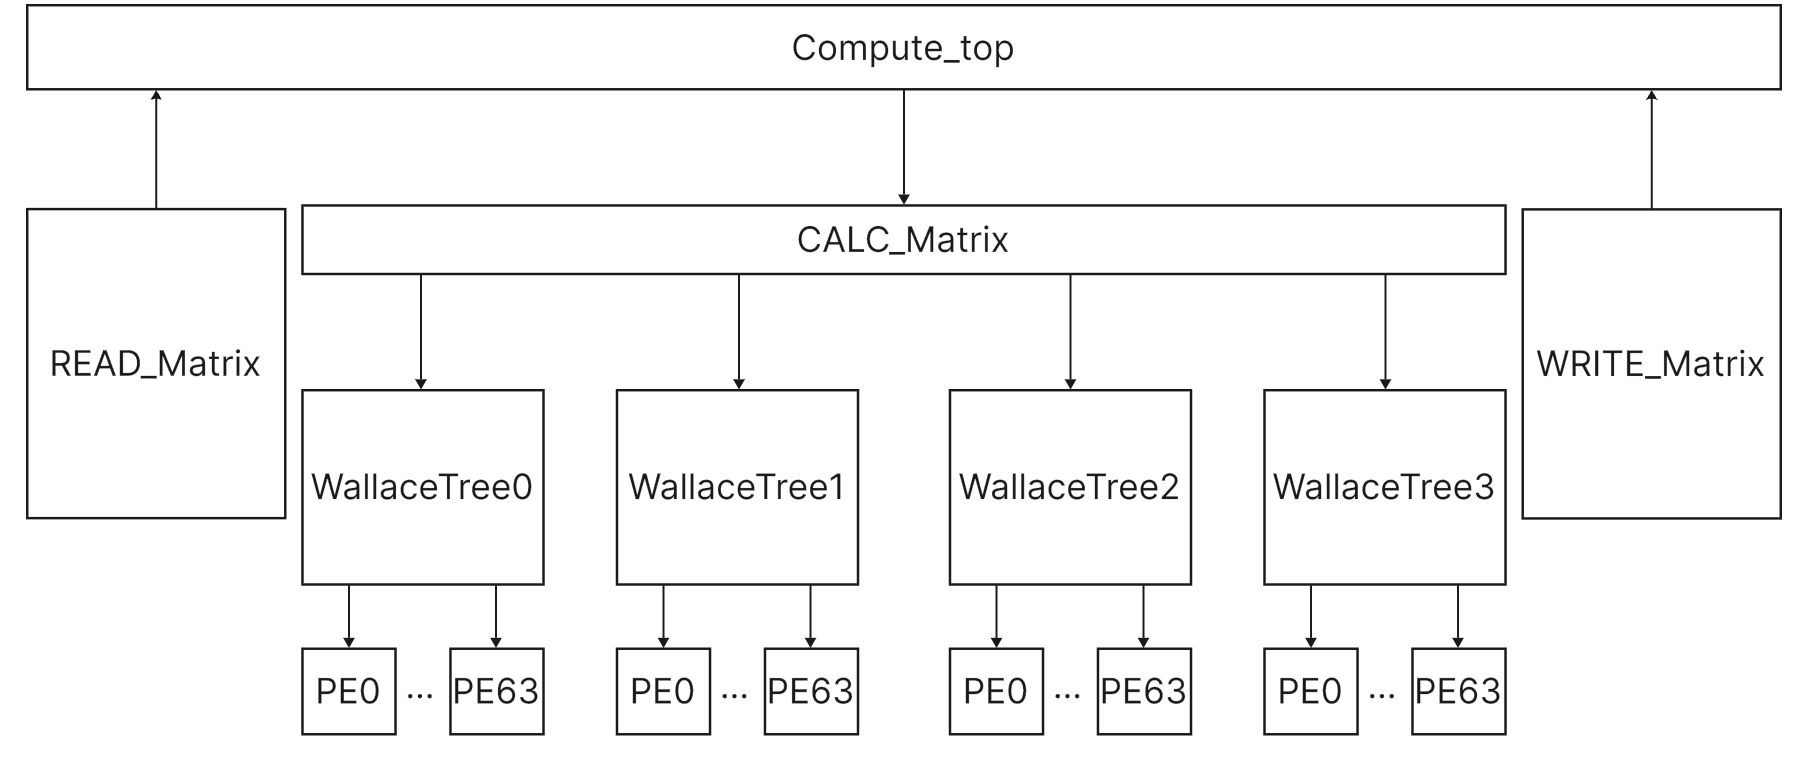
\includegraphics[width=\linewidth]{fig/mixed.png}
		\caption{混合精度矩阵乘法模块架构}
		\label{fig:mixed}
	\end{figure}
	
	在 CPU–FPGA 耦合 VLM 推理系统中，另一个关键挑战在于如何高效支持混合精度量化模型的推理计算。近年来，为降低大规模 Transformer 模型的存储与计算开销，INT4、INT8 以及 FP16 等低精度量化方式被广泛应用于 VLM 推理部署。然而，不同模块往往具有不同的数值敏感性：例如，Attention 中部分累加操作通常需要较高精度以保证数值稳定性，而 MLP 与线性投影层则更适合采用低比特量化以减少存储与带宽开销。因此，实际推理过程中往往需要在不同精度模式之间动态切换，这对 FPGA 计算架构提出了较高要求。
	
	传统 FPGA 推理加速器通常针对单一精度进行定制设计，其 DSP 数据通路、乘加结构以及缓存布局均固定于某一种数值格式。当模型中同时存在 INT4、INT8 与 FP16 运算时，若分别构建独立计算模块，不仅会导致大量逻辑资源冗余，还会增加数据调度与流水线控制复杂度；而若直接采用高精度统一计算，则又会削弱低比特量化带来的吞吐率与功耗优势。因此，如何在统一硬件架构下兼容多种量化精度，并在资源受限 FPGA 上实现高吞吐矩阵乘法，成为混合精度推理系统设计中的核心问题。
	
	针对上述挑战，本文设计了一种 Mixed-precision Matrix Multiplication Architecture。该架构在 FPGA 上构建统一的整型与浮点计算通路，通过可重构数据路径与参数化乘加树结构，实现 INT4、INT8 与 FP16 三种精度模式的统一支持，从而满足 VLM 推理过程中不同算子的混合精度计算需求。
	
	具体而言，系统首先设计了可配置输入解码模块（Precision-aware Decode Unit），用于根据当前计算模式动态解析不同位宽的数据格式。在 INT4 与 INT8 模式下，输入数据会被打包存储于统一缓存结构中，通过位宽切分逻辑动态提取对应整数数据；而在 FP16 模式下，则采用浮点尾数与指数并行解析方式恢复标准半精度浮点表示。通过统一的数据入口设计，系统能够在不改变整体数据流结构的前提下实现不同精度间的快速切换。
	
	在乘加计算部分，本文提出了一种参数化 MAC Tree（Multiply-Accumulate Tree）结构。与传统固定精度 DSP 链不同，该 MAC Tree 能够依据当前精度模式动态调整内部计算粒度。在 INT4 模式下，单个 DSP 可同时执行多个低比特并行乘法，从而提高单位周期吞吐率；在 INT8 模式下，则采用标准整数乘加流水线执行计算；而在 FP16 模式下，系统启用浮点乘法与指数对齐逻辑，以保证高精度 Attention 与归一化计算的数值稳定性。
	
	为了进一步提升矩阵运算吞吐率，系统在 FPGA 上实例化了 4 组独立运行的乘加树阵列（MAC Tree Array）。每个阵列内部集成 64 组可流水线化执行的 MAC Tree Processing Element，并采用二维规则互连结构构建局部矩阵乘法计算网络。整体上，4 个阵列共同形成一个 16×16 的矩阵乘法计算阵列，可同时处理多个 token 与权重块的数据计算任务。
	
	在执行过程中，输入矩阵数据会被划分为多个 tile，并通过片上 Buffer 分发至不同 MAC Tree 阵列。各阵列内部采用深流水线结构实现矩阵分块计算：前级负责输入加载与精度解码，中间级执行并行乘加运算，后级完成部分和累积与结果写回。由于不同阶段能够并行工作，因此系统能够有效隐藏数据搬运延迟，并持续保持 DSP 阵列高利用率。
	
	此外，针对混合精度场景下不同数据格式间的数据对齐问题，系统进一步设计了统一的 Accumulation Buffer 与 Precision Control Scheduler。前者用于对不同精度模式下的部分和结果进行统一缓存与归约；后者则负责在 Transformer 不同算子之间动态切换计算模式。例如，在 MLP 层中可优先采用 INT4/INT8 模式提升吞吐率，而在 Softmax 与 LayerNorm 等对数值敏感的模块中则切换至 FP16 模式，以保证整体模型精度。
	
	相比传统单精度 FPGA 加速器，本文提出的混合精度矩阵乘法架构具有三个显著优势。首先，其通过统一数据通路兼容多种量化精度，避免了为不同精度重复构建独立硬件模块所带来的资源浪费；其次，参数化 MAC Tree 能够充分利用低比特量化下的 DSP 并行能力，从而显著提升单位周期计算吞吐率；最后，该设计支持运行时动态精度切换，使系统能够根据不同 Transformer 算子的数值特性灵活选择最优计算模式，在保证模型精度的同时有效降低推理延迟与功耗开销。
	
	\section{量化 VLM 模型 MLP 参数稀疏性预测器}

	第二个挑战在于如何在推理过程中动态预测模型参数的稀疏性，从而进一步减少冗余计算。为此，项目针对模型的 MLP 中间层参数设计了一种基于输入特征的分组稀疏预测器。该预测器旨在通过极低的额外计算开销，预先识别并屏蔽对输出表征贡献较小的中间层神经元，从而实现计算路径的动态无结构剪枝与硬件加速。
	
	\subsection{分组策略与监督目标}

	在大语言模型与大规模 ViT 的标准架构中，MLP 层的中间层维度 $d_{\mathrm{ff}}$ 通常远大于输入特征维度 $d$。为了在硬件实现效率与预测粒度之间取得最佳平衡，本文采用静态索引分组策略。具体而言，我们将中间层通道按索引连续划分为 $G$ 个不重叠的组，每组包含 $m$ 个通道，即 $G = d_{\mathrm{ff}} / m$。对于任意组 $j \in \{0, 1, \dots, G-1\}$，其包含的通道索引集合定义为 $\mathcal{G}_j = \{i \in \mathbb{Z} \mid jm \le i < (j+1)m \}$。
	
	预测器的监督信号源自真实前向传播过程中的激活强度。对于给定的输入标记特征向量 $x$，其穿过 MLP 第一层线性映射并经由非线性激活函数后得到的输出为 $h = \sigma(W_1 x)$。我们定义第 $j$ 组的重要性评分 $g_j$ 为该组内所有神经元激活绝对值的算术平均值：
	\begin{equation}
		g_j = \frac{1}{m}\sum_{i \in \mathcal{G}_j} |h_i|
	\end{equation}
	
	随后，对全局评分进行最大值归一化处理，即 $\tilde{g}_j = g_j / \max(g)$。为生成硬监督信号，我们选取评分排名前 $k$ 的组生成二值化掩码标签 $y_j^{*} \in \{0, 1\}$：
	\begin{equation}
		y_j^{*} = \mathbf{1}[j \in \mathrm{TopK}(\tilde{g}, k)]
	\end{equation}
	此种基于 $\mathrm{Top\text{-}}k$ 机制的监督范式，确保了预测器能够精准捕捉并学习每一层中最具代表性的高维特征响应模式。
	
	\subsection{预测器架构与前向推理}

	针对 CLIP Vision Tower 的每一层 Transformer Block，我们均实例化并独立训练一个线性预测头。其输入为经由 LayerNorm 归一化处理后的标记特征 $x \in \mathbb{R}^d$，输出为该层各组的预测得分向量 $s \in \mathbb{R}^G$：
	\begin{equation}
		s = W^{(p)} x + b^{(p)}
	\end{equation}

	其中，$W^{(p)} \in \mathbb{R}^{G \times d}$ 与 $b^{(p)} \in \mathbb{R}^G$ 分别为预测器的可学习权重矩阵与偏置向量。在训练阶段，模型采用二元交叉熵损失函数来最小化预测概率 $\hat{y}_j = \sigma(s_j)$ 与目标真实掩码 $y_j^{*}$ 之间的分布差异：
	\begin{equation}
		\mathcal{L} = \sum_{j=0}^{G-1} \mathrm{BCE}(\hat{y}_{j}, y_{j}^{*})
	\end{equation}
	
	在实际推理部署阶段，预测器基于推断得分直接生成硬件执行掩码 $M_j$：
	\begin{equation}
		M_j = \mathbf{1}[j \in \mathrm{TopK}(s, k_{\mathrm{infer}})]
	\end{equation}

	该掩码 $M_j$ 被直接旁路至底层硬件调度单元，动态触发对应组别的参数块参与后续的高密矩阵乘法运算，从而达成细粒度稀疏计算。为增强预测器在极稀疏场景下的泛化与鲁棒性，我们在训练与推理阶段采用解耦的 $k$ 值设定（即 $k_{\mathrm{train}} > k_{\mathrm{infer}}$）。这种解耦设计能有效规避在目标稀疏度极高时，因正负样本标签（1 与 0）比例严重失衡而导致的预测器训练收敛困难问题，通过在训练阶段引入更丰富的梯度信号，显著提升了预测器对稀疏激活模式捕捉的稳健性。
	
	\subsection{动态层级稀疏度调度}

	鉴于 ViT 在深浅层特征提取重心的内在差异（浅层侧重局部纹理细节，深层聚焦全局高阶语义），本文进一步引入了动态层级 $k$ 值调度机制。该机制允许根据网络层所处的阶段（如浅层、中层、深层）动态调整保留比例 $\gamma$。此外，为适配硬件流水线的对齐需求，最终确定的各层 $k$ 值需满足与硬件有关的位宽对齐规范，以确保理论上的稀疏度能够转化为实际的计算加速。
	
	\section{面向稀疏矩阵乘法的加速架构}
	
	第三个挑战在于如何高效执行稀疏矩阵乘法计算。由于稀疏模型中大量权重为零，若仍采用密集矩阵计算方式，将无法充分利用稀疏性带来的性能优势。面对该问题，项目在 FPGA 上设计了一种专用的稀疏矩阵乘法计算单元：该单元结合稀疏性预测器生成的 mask 向量以及 token 维护信息（用于标记 token 数值是否超过预设阈值），从原始稀疏矩阵中动态提取参与计算的若干密集子矩阵，并将其重构为标准矩阵形式后输入乘加树阵列执行矩阵乘法运算，得到输出结构后对其进行解封装以生成输出 token，并同步更新 token 维护信息。该设计有效避免了无效零元素对乘加资源的占用，显著降低了乘加操作数量，从而提升了整体推理计算效率。
	
	\subsection{稀疏性预测器硬化电路}
	
	神经元稀疏性预测器采用 FP16 精度的单层感知器神经网络结构。为了最大程度降低 CPU 与 FPGA 之间的数据传输带宽压力，Ordovician 将稀疏性预测器直接硬化部署在 FPGA 电路中，并作为稀疏矩阵乘法模块的核心子模块，其整体结构如图\ref{fig:predictor}所示，由计算电路与参数存储两部分组成。
	
	\begin{figure}[htbp]
		\centering
		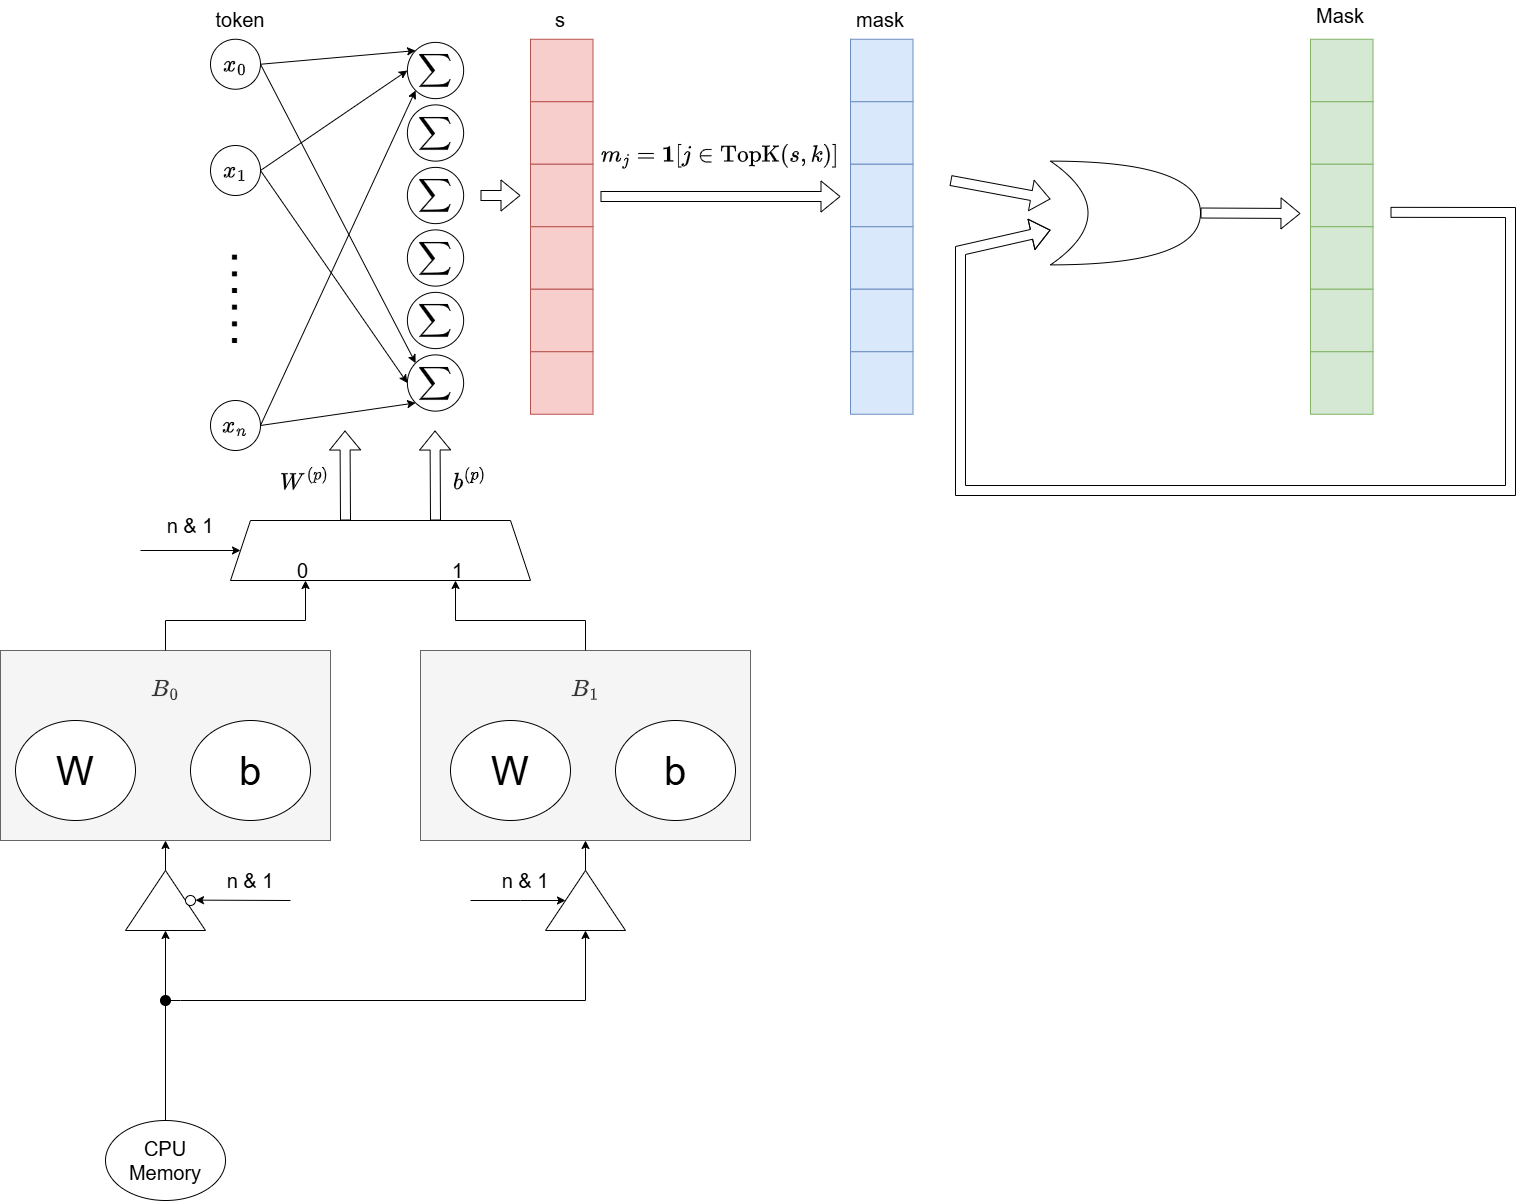
\includegraphics[width=0.8\columnwidth]{fig/predictor_architecture.png}
		\caption{Predictor Architecture.}
		\label{fig:predictor}
	\end{figure}

	\textbf{计算电路}
	计算电路负责对输入 token 向量执行稀疏性预测计算。输入 token 首先与对应的权重矩阵和偏移向量进行线性变换，该过程直接基于 FPGA 内部 DSP 单元实现，从而生成当前层的预测 mask 向量；随后，该预测 mask 向量再与当前 Transformer Block 对应的 Mask 向量执行或运算，最终得到用于控制后续稀疏矩阵乘法计算的稀疏激活向量。

	\textbf{参数存储}
	参数存储部分则用于保存各个 Transformer Block 离线训练得到的预测器权重与偏移参数。考虑到 FPGA 片上存储资源有限，Ordovician 将预测器参数存储于 FPGA 的 URAM 中，并设计了双缓冲参数管理机制以隐藏参数传输延迟。Ordovician 在 FPGA 内部实例化了两组参数存储空间 $B_0$ 与 $B_1$，在 FPGA 启动阶段，CPU 首先向 $B_0$ 写入 $Block_0$ 对应的预测器参数；当 FPGA 使用 $B_0$ 中的数据执行 $Block_0$ 推理计算时，CPU 会并行向 $B_1$ 写入 $Block_1$ 的参数；随后，在 $Block_1$ 推理阶段，FPGA 切换至使用 $B_1$ 中的数据，而 CPU 则继续向 $B_0$ 写入 $Block_2$ 的参数。以此类推，当系统执行 $Block_n$ 推理时，FPGA 始终读取 $B_{n\%2}$ 中的数据，而 CPU 则同步向 $B_{(n+1)\%2}$ 中写入 $Block_{n+1}$ 对应参数。
	
	通过这种交替读写的双缓冲参数管理策略，Ordovician 能够在少量片上存储开销下实现预测器参数的持续流式更新，使参数传输过程与 Transformer 推理计算过程相互重叠，从而有效隐藏稀疏性预测器的 CPU/FPGA 数据传输延迟，进一步提升整体稀疏推理系统的执行效率。
	
	\subsection{稀疏矩阵乘法模块}
	
	在稀疏化 VLM 推理过程中，仅依赖神经元级稀疏预测仍无法充分发挥模型稀疏性带来的性能优势。虽然稀疏性预测器能够提前筛除大量非激活神经元，但传统矩阵乘法计算仍通常以完整稠密矩阵为输入，导致 FPGA 计算阵列在执行过程中仍需遍历大量无效零值数据。这不仅浪费 DSP 乘加资源，还会带来额外的片外存储访问与数据搬运开销。因此，如何在 FPGA 上高效执行动态稀疏矩阵乘法，并避免传统稀疏格式带来的复杂控制逻辑，成为提升整体推理效率的关键问题。
	
	Ordovician 设计了一种面向动态 Transformer 稀疏性的 稀疏矩阵乘法架构，其整体流程如图\ref{fig:sparse_multiplication}所示。该设计结合稀疏性预测器生成的神经元激活 Mask 向量与模块维护的 Token 状态表，在运行时动态提取有效矩阵区域，并重构为适合 FPGA 流水线执行的局部稠密子矩阵，从而实现高效的稀疏矩阵乘法计算。
	
	\begin{figure}[htbp]
		\centering
		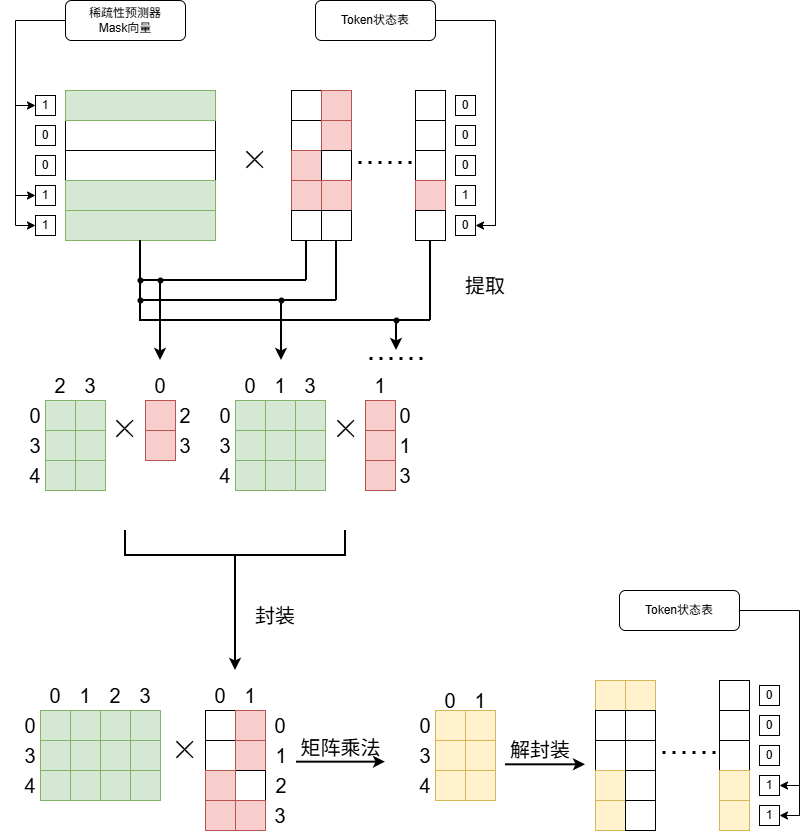
\includegraphics[width=0.8\columnwidth]{fig/sparse_matrix_multiplication_architecture.png}
		\caption{Sparse Matrix Multiplication Architecture.}
		\label{fig:sparse_multiplication}
	\end{figure}
	
	具体而言，在进入 MLP 推理阶段后，系统首先由稀疏性预测器生成当前层的 Mask 向量，用于标识哪些输出神经元会被激活。如图左上部分所示，mask 中值为 1 的行对应需要参与当前计算的神经元，而值为 0 的部分则被直接跳过。与此同时，系统维护 Token 状态表，用于记录输入 token 各维度是否超过预设阈值。图中右侧的 Token 状态表表明，仅部分 token 通道被认为具有有效贡献，其余低贡献维度将不再参与后续乘加运算。
	
	随后，矩阵提取模块根据上述两类稀疏信息，对原始矩阵执行双维度动态裁剪。一方面，仅保留被 Mask 向量激活的矩阵行；另一方面，仅保留 Token 状态表中标记为有效的输入列。图中红色区域表示被筛选出的有效元素，而白色部分则被直接忽略。Ordovician 通过这种“行—列联合过滤”机制，能够同时利用神经元级与 token 级稀疏性，大幅减少实际参与计算的数据规模。
	
	然而，动态提取后的矩阵片段在存储布局上通常是不连续且不规则的，难以直接映射到 FPGA 的规则矩阵乘法阵列。因此，系统进一步设计了矩阵封装单元，对提取出的稀疏片段进行在线重构。如图中部所示，原始不规则矩阵区域被重新组织为多个连续存储的局部稠密子矩阵，并同步生成对应的输入 token 子向量，使后续计算能够采用标准流水线矩阵乘法结构执行。
	
	在计算阶段，重构后的局部稠密子矩阵会被送入 FPGA 上的混合精度乘法阵列。由于大量无效零元素已在前级被剔除，乘加树仅需执行真实有效数据对应的乘加运算，从而显著提高 DSP 利用率与流水线吞吐率。图中下部展示了重构后的小规模稠密矩阵与 token 子向量，其计算结果最终形成局部输出结果矩阵。
	
	完成局部矩阵乘法后，系统通过矩阵解封装模块将局部输出重新映射回原始 token 空间。如图右下部分所示，局部计算结果会依据之前保存的索引关系恢复至完整输出结构，同时同步更新 Token 状态表，用于后续 Transformer Block 的动态稀疏推理。对于未参与计算的位置，系统默认填充为零，从而保证最终输出 token 的结构一致性。
	
	与传统稠密矩阵乘法相比，Ordovician 提出的面向稀疏矩阵乘法的加速架构具有三个关键优势。首先，其能够同时利用神经元级与 token 级动态稀疏性，进一步降低实际参与计算的数据规模；其次，该设计无需运行时执行复杂的 CSR/CSC 稀疏格式转换，避免了额外控制开销；最后，通过局部稠密重构机制，系统能够充分适配 FPGA 的规则流水线与矩阵乘法阵列结构，从而在资源受限环境下实现低延迟、低功耗的 VLM 推理加速。
	
	\section{Implementation}
	
	Ordovician 系统实现分为算法层面的稀疏性预测器训练与硬件层面的 CPU/FPGA 推理计算通路设计。
	
	\subsection{预测器训练}
	
	\textbf{软硬件环境。}
	本研究的所有实验均在配备单张 NVIDIA A10 GPU（24GB 显存）的服务器上执行。底层软件栈基于 PyTorch 2.7.1 深度学习框架构建，并适配 CUDA 11.8 加速环境。
	
	\textbf{基座模型与数据预处理。}
	视觉基座模型采用 QVLM 的视觉编码器（初始化自 \texttt{openai/clip-vit-large-patch14}），其包含 24 层 Transformer Block，特征嵌入维度 $d=1024$，前馈网络中间层维度 $d_{\mathrm{ff}}=4096$。在视觉特征提取阶段，严格遵循 CLIP 官方预处理协议：输入图像首先经由双三次插值缩放至短边 224 像素，随后进行 $224 \times 224$ 的中心裁剪，并利用标准均值 $(0.481, 0.458, 0.408)$ 与标准差 $(0.269, 0.261, 0.276)$ 完成像素级归一化。
	
	\textbf{数据与监督信号。}
	预测器的训练与校准基于 ScienceQA 数据集的 QCM-LEPA 子集（共 4241 个样本）展开。在训练过程中，我们冻结 Vision Tower 的主干参数，仅通过单次前向传播提取每一层 MLP 的激活值（\texttt{act}）作为密集计算的监督信号。具体而言，基于真实激活强度的 Top-$k$ 分布生成目标掩码，将预测任务建模为二元交叉熵分类问题。
	
	\textbf{预测器架构。}
	针对 Vision Tower 的每一层，我们实例化了一个线性预测头。其输入为 \texttt{layer\_norm2} 输出的 Token 特征。采用组大小 $m=64$ 的分组策略，将 4096 维的中间层连续划分为 64 组（即预测输出维度为 64），并通过均值池化聚合组内评分。
	
	\textbf{稀疏度调度策略。}
	为平衡网络深度的特征表征需求与底层硬件调度效率，我们实施了层级 $k$ 值调度机制。Vision Tower 的 24 层被均匀划分为三个阶段：
	\begin{itemize}
		\item \textbf{浅层与深层（第 0-7 层，第 16-23 层）：} 采用较为保守的稀疏保留比例（$k_{\mathrm{ratio}}=0.3$）。
		\item \textbf{中层（第 8-15 层）：} 施加更激进的稀疏约束（$k_{\mathrm{ratio}}=0.2$）。
	\end{itemize}

	上述配置生成的各层理论 $k$ 值，均以 $k_{\mathrm{align}}=128$ 为粒度进行对齐取整。为增强预测器在极度稀疏条件下的鲁棒性，我们在训练和推理阶段解耦了 $k$ 值参数，即训练时提供相对稠密的监督信号（$k_{\mathrm{train}}=1024$），而推理阶段则严格执行高稀疏掩码（$k_{\mathrm{infer}}=256$）。
	
	\begin{figure}[htbp]
		\centering
		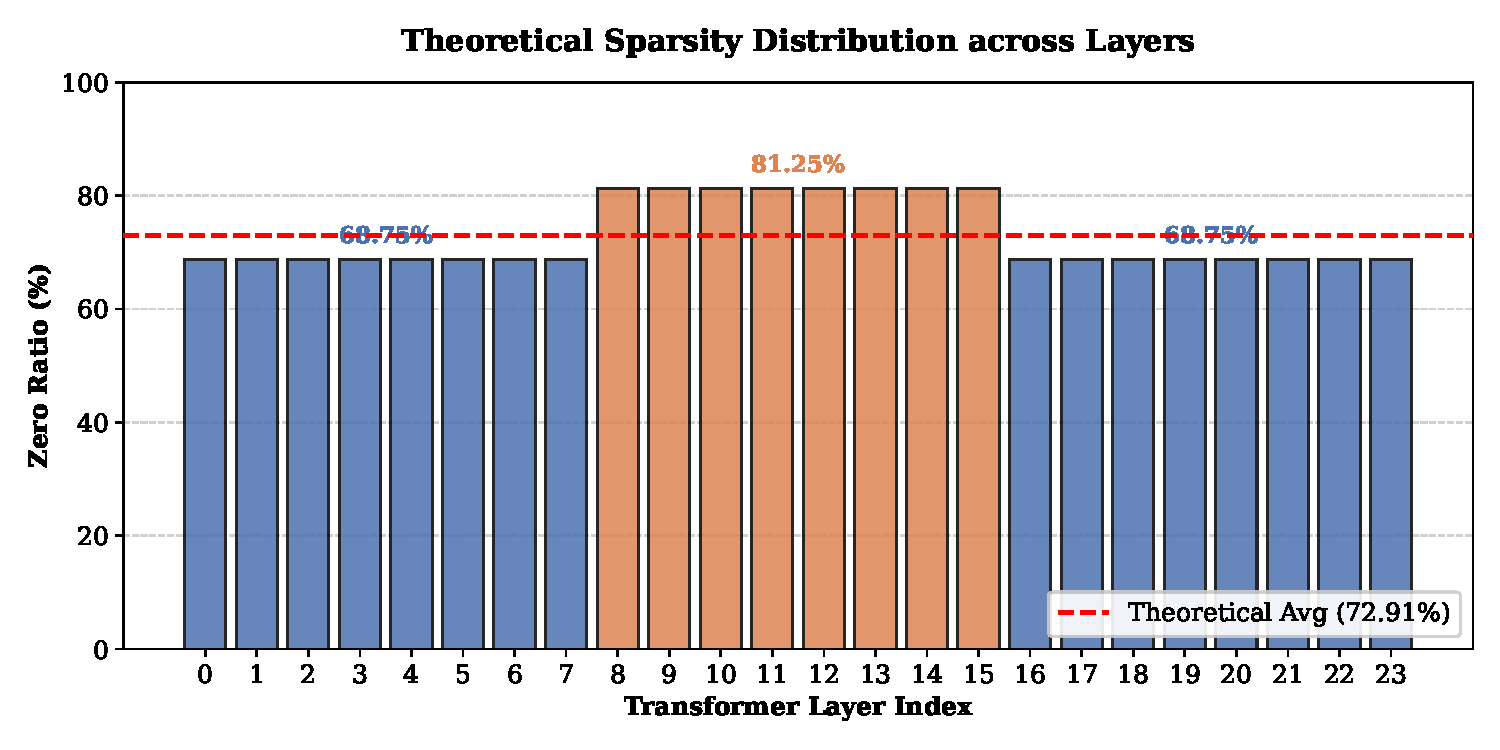
\includegraphics[width=\linewidth]{fig/layerwise_sparsity_distribution.pdf}
		\caption{Theoretical Sparsity Distribution across Layers. 鉴于对齐规范（$k_{\mathrm{align}}=128$），中层（第8-15层）展现出比浅层与深层更激进的参数削减幅度，全网理论平均稀疏度达到 72.91\%。}
		\label{fig:layerwise_sparsity}
	\end{figure}
	
	\textbf{模型优化。}
	模型优化采用简单的随机梯度下降算法，初始学习率设定为 $\text{lr}=1 \times 10^{-2}$，动量（Momentum）为 $0.9$。在训练策略上，设置单次前向的微批次大小为 1，并配合梯度累积技术，每 8 个样本（\texttt{update\_every=8}）执行一次参数更新。模型共计在 6218 个图像样本上进行了训练（对应约 777 次优化器步进）。在此配置下，稀疏模型在 ScienceQA 全量任务上的精度仅比全量推理的基线下降约 0.61\%，验证了该方案在极低精度损失下实现高效计算的潜力。
	
	\subsection{计算通路设计}

	在硬件层面，Ordovician 基于 Vitis 构建了完整的 Transformer 推理计算通路，实现了从输入 token 到输出 token 的端到端 VLM 推理流程
	
	\text{FPGA 侧。}
	Ordovician 采用 Vitis HLS 设计工具，以 VLM 中 Full Self-Attention Transformer Block 为基础，为 MHA 与 MLP 模块分别构建了支持混合精度计算的矩阵乘法阵列，并针对 MLP 层广泛存在的激活稀疏性，进一步设计实现了稀疏性预测器与稀疏矩阵乘法计算架构。除 Transformer 核心矩阵运算模块外，Ordovician 还针对不同精度数据在推理过程中的数值计算需求，分别为 LayerNorm、GELU 以及 Residual Connection 关键算子设计了独立的数据通路与计算模块，从而保证 INT4、INT8 与 FP16 混合精度数据能够在统一硬件架构下稳定、高效地完成推理计算。
	
	\textbf{CPU 侧。}
	为实现 CPU/FPGA Co-Processing 协同执行机制，Ordovician 基于 Vitis Software Application 开发流程，采用 C++ 与 XRT 库实现了 host.cpp 程序。host.cpp 对外负责提供模型推理所需的数据交互接口以及模型参数地址管理功能，对内则负责 FPGA 加速算子的启动控制和 CPU/FPGA 间的数据流调度，从而实现 FPGA 推理计算与 CPU 控制逻辑之间的协同运行。
	
	此外，为满足 FPGA 加速器对模型参数细粒度、高带宽访问的需求，Ordovician 还额外开发了若干 Python 数据预处理脚本，用于从原始模型权重文件中提取不同 Transformer Block 及不同 Transformer 阶段对应的参数数据，并进一步将其转换为适用于 FPGA 侧传输的 .dat 格式文件。
	
	目前，Ordovician 已面向 LLaVA-7B 模型的 Vision Tower 部分，在 Kria KV260 Vision AI Starter Kit 平台上完成推理部署，并基于 Vitis 2025.2 完成了 C/RTL Co-Simulation 以及 HLS Synthesis/Implementation 的完整验证流程，验证结果表明系统能够正确完成混合精度 Transformer 推理计算，并具备进一步扩展至完整 VLM 推理部署的能力。
	
	\section{Evaluation}

	\subsection{预测器性能评估}
	
	本节我们对视觉稀疏预测器的性能及其对端到端多模态任务的影响进行全面评估。评估主要围绕预测器自身的离线特征捕捉能力、极致稀疏下的计算缩减率，以及在 ScienceQA 问答任务上的端到端性能表现展开。
	
	\subsubsection{预测器离线特征评测}
	为了验证分组稀疏预测器对真实激活掩码的拟合能力，我们在包含 64 个图像样本的离线验证集上进行了细粒度评估。在设定的高稀疏推理配置（$k_{\mathrm{infer}}=256$）与层级调度机制下，预测器展现出了出色的分类性能。
	
	实验结果表明，预测生成的掩码与真实激活 Top-$k$ 掩码之间的 \textbf{F1-Score达到了 0.6548}，\textbf{Jaccard 相似度达到了 0.4971}。值得注意的是，与完全随机生成掩码的基线相比，本方法实现了 \textbf{1.4176 倍的 F1 性能提升}。这有力地证明了预测器并未退化为均匀采样，而是精准捕捉到了 Vision Tower 内部与图像语义强相关的关键神经元激活模式。
	
	\subsubsection{特征稀疏度与保真度分析 }
	实现高效推理的核心在于最大化屏蔽冗余参数运算，同时保留核心特征表征。我们在全层范围内对预测器生成的掩码效应进行了统计分析。
	
	结果显示，在此配置下，模型实现了高达 72.63\% 的平均激活零值比例。值得注意的是，根据我们的层级稀疏度调度策略（即首尾阶段比例为 0.3，中段为 0.2，且严格遵循 128 对齐原则），Vision Tower 各层的理论零值分布为：浅层与深层各 68.75\%，中层为 81.25\%。由此计算出的全网理论平均零值比例为：
	\begin{equation}
		\frac{8 \times 68.75\% + 8 \times 81.25\% + 8 \times 68.75\%}{24} \approx 72.91\%
	\end{equation}
	这一理论期望值与我们端到端真实评测所得的 72.63\% 高度一致。二者之间微小的误差主要源于输入序列中特殊标记（如 \texttt{[CLS]} Token 或 Padding 区域）未完全参与掩码计算。这种高度的理论与经验一致性，不仅验证了动态层级调度策略在代码层面的精准执行，也凸显了该方法在实际硬件部署时，对显存占用和计算加速具有极高的可预测性。
	
	与此同时，掩码作用后的输出特征与未剪枝的原始特征之间的\textbf{余弦相似度保持在 0.1578}。尽管绝对相似度数值受极高稀疏度的影响存在一定偏移，但后续的端到端评测表明，这种特征空间的稀疏映射并未对高阶语义产生破坏性影响。
	
	\subsubsection{ScienceQA 端到端性能评测 }
	为了量化稀疏化对基座视觉语言模型（QVLM）实际问答能力的冲击，我们在 ScienceQA 测试集的 QCM-LEPA 子集（共包含 4241 个问题）上进行了全量评估。
	
	测试结果显示，采用全参数密集推理的基线模型（Baseline）在该测试集上的准确率为 \textbf{40.8630\%}（1733/4241）。而部署了动态视觉稀疏预测器的掩码模型（Masked Model），在削减了约 72\% MLP 计算量的前提下，依然维持了 \textbf{40.2499\%}（1707/4241）的准确率。整体精度损失仅为 \textbf{$-0.6131$ 个百分点}。这一微小的性能衰减充分证明了所提预测器架构在“激进压缩计算开销”与“维持多模态推理能力”之间取得了极佳的平衡。
	
	\begin{table}[htbp]
		\centering
		\begin{threeparttable}
			\caption{ScienceQA 数据集上的端到端性能与稀疏度对比。}
			\label{tab:main_results}
			\begin{tabular}{lcccc}
				\toprule
				\textbf{Method} & \textbf{Acc (\%)} & \textbf{$\Delta$ Acc} & \textbf{Zero Ratio (\%)} & \textbf{F1 Score} \\
				\midrule
				Baseline (Dense)\tnote{*} & 40.86 & --- & 0.00 & --- \\
				\textbf{Ours (Predictor)} & \textbf{40.25} & \textbf{$-$0.61} & \textbf{72.63} & \textbf{0.6548} \\
				\bottomrule
			\end{tabular}
			\begin{tablenotes}
				\small
				\item[*] 注：基线模型（Baseline）采用全参数密集推理，不涉及动态特征掩码预测过程，故不报告 F1 分数与掩码零值比例。基线模型的真实激活分布仅作为计算预测器 F1 性能的相对真值。
			\end{tablenotes}
		\end{threeparttable}
	\end{table}
	
	\section{Conclusion}
	
	\section{Acknowledgments}


	\begin{small}
		\bibliography{pa}
		\bibliographystyle{plain}
	\end{small}
	
\end{document}